%!TEX root = ../thesis.tex

\begin{savequote}[60mm]
	There's no reason to have a plan B\\
	because it distracts from plan A.
	\qauthor{Will Smith}
\end{savequote}

\chapter{Experimental results}\label{chapter:results}
	
	This chapter expands the previous one by verifying the usability of Open LoRa Mesh.
	Particularly, it describes four experiments in which Open LoRa Mesh has been set up and tested, in order to record its rough performances.The following sections describe such experiments done with the available hardware in two particular locations: inside a building and in an open field.
	
	The first location is \textit{Archimedes Tower} \footnote{ For simplicity, pictures representing this location are taken from a publicly available online 3D model\newline (\url{https://3dwarehouse.sketchup.com/model/a4d327dd45162ee0557d96e459f19076/})} (\textit{Torre Archimede} in Italian), the building which houses the department of mathematics and computer science at the University of Padova, while the second place is the \textit{Mazzini Square} \footnote{ Images of this location in this thesis are taken from Google Maps and OpenStreetMap} (\textit{Piazza Mazzini} in Italian) in Monselice, a city in the south of Padova.
	
	These places have been chosen especially for their opposite characteristics: Archimedes Tower, in Figure~\ref{img:archimede_1}, is a 31m tall building which develops on seven levels above the ground and three underground levels\footnote{ \url{https://phaidra.cab.unipd.it/view/o:10783}}, while Mazzini Square, in Figure~\ref{img:pzza_mazzini_1}, is an open space that allows an unobstructed view between nodes.
	
	An important remark that has to be done before describing these experiments is that they are not exhaustive.
	When thinking about the amount of possibilities in which nodes can be arranged, it is certain that more tests could have been executed.
	Such kind of system testing has to take in consideration also the surroundings of devices, since they communicate wirelessly.
	
	\begin{minipage}{0.5\textwidth}%
		\begin{figure}[H]
			\centering
			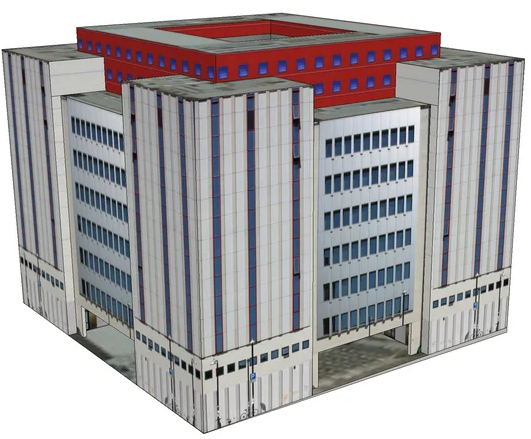
\includegraphics[width=\textwidth]{resources/img/chap5/archimede_1}
			\caption{3D model of Archimedes Tower}
			\label{img:archimede_1}
		\end{figure}
	\end{minipage}%
	\hfill%
	\begin{minipage}{0.5\textwidth}\raggedright
		\begin{figure}[H]
			\centering
			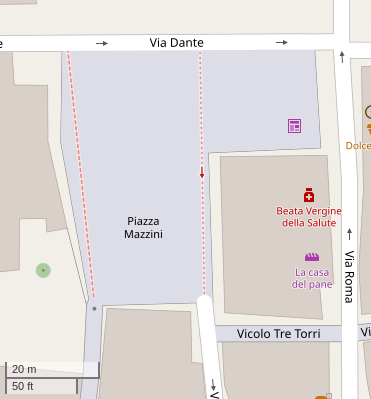
\includegraphics[width=.8\textwidth]{resources/img/chap5/pzza_mazzini_1}
			\caption{View from above of Mazzini Square}
			\label{img:pzza_mazzini_1}
		\end{figure}
	\end{minipage}%
	
	\section{Board placement}
	
		For these experiments, all four boards have been used to test the functionalities of the network.
		Placement of the boards is represented for both locations, respectively in Figure~\ref{img:archimede_2} for Archimedes Tower and in Figure~\ref{img:pzza_mazzini_2} for Mazzini Square.
		
		\begin{figure}[h]
			\centering
			\includegraphics[width=.6\textwidth]{resources/img/chap5/archimede_2}
			\caption{Placement of boards in Archimedes Tower}
			\label{img:archimede_2}
		\end{figure}
	
		Regarding Archimedes Tower, boards have been placed so that board \textbf{\textit{A}} is on the 6$^{th}$ floor, \textbf{\textit{B}} is on the 4$^{th}$ floor, \textbf{\textit{C}} is on the 2$^{nd}$ floor, \textbf{\textit{D}} is on the first underground level.
		All boards have been placed with the antenna facing the internal courtyard of the building.
		
		For Mazzini Square, on the other hand, boards have been placed so that they are directly visible to each other, almost one for each corner of the square.
		
		\begin{figure}[h]
			\centering
			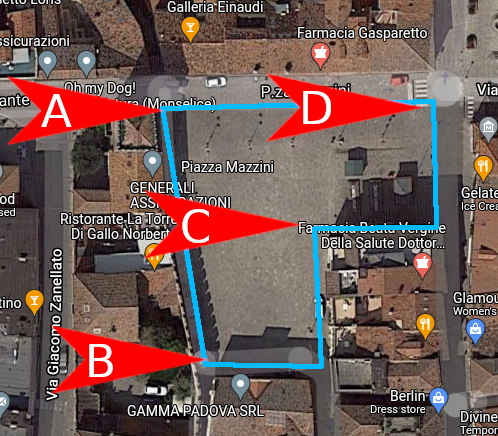
\includegraphics[width=.75\textwidth]{resources/img/chap5/pzza_mazzini_3}
			\caption{Placement of boards in Mazzini Square}
			\label{img:pzza_mazzini_2}
		\end{figure}
	
		These placements have been made so that boards do not have direct obstructions that can block the signal in between them.
		Such placement can be considered ideal because nodes are not far from one another, and their signal does not lose much power.

		In both scenarios boards have been tested as if they were part of a network of fixed devices, which, as explained in Section~\ref{sec:fixed_network}, is the best case scenario for Open LoRa Mesh.
	
	\section{Experiments}
		
		Following there are the four experiments done to test the usability of the network: \textit{message range}, \textit{mesh creation}, \textit{node addition} and \textit{node removal}.
		These sections contain a description on how these experiments have been executed and the results achieved.
		
		\subsection{Message range}
		
			This first experiment is intended to understand nodes' range and how they can be placed in order to achieve a strongly connected network.
			
			In the case of Archimedes Tower, this test has shown the weakness of LoRa when devices are placed inside a building.
			Considering the placement of nodes as represented in Figure~\ref{img:archimede_2}, various cases have been examined.
			
			To test the transmission range of the nodes in the worst-case scenario, at first device \textbf{\textit{D}} has been booted on the library's floor.
			After booting up, the device listens for around 180 seconds for any mesh advertisement messages, as explained in Section~\ref{subsec:initialization}, but since there are no other nodes on it will create a new mesh with the specified identifier.
			Subsequently, device \textbf{\textit{A}} was the second one started, but, due to the number of concrete layers in between these devices, not all packets were correctly exchanged in between these two nodes.
			This has caused device \textbf{\textit{A}} not being able to exchange data with node \textbf{\textit{D}} and to be shut down so that a better placed node could be booted up.
			Node \textbf{\textit{B}}, placed on the 4$^{th}$ floor, showed better results when exchanging mesh data, although some messages were still lost when communicating with node \textbf{\textit{D}}.
			
			The best placement of nodes in Archimedes Tower is thus represented by the placement in Figure~\ref{img:archimede_1}.
			Nodes have shown a strong connection when placed roughly two levels apart and booted up in order, allowing the mesh to be created without any packet loss.
			FiPys have been booted in alphabetical order and two minutes apart from each other, so the first one would have time to generate the mesh, and the others would be able to join it.
			The addition of a node is further described in Section~\ref{subsec:node_addition}.
			
			Contrasting with the thick walls of Archimedes Tower, Piazza Mazzini is an open space where no obstructions are present.
			In this scenario, whatever is the order in which devices are booted, all of them have a clear line of sight with one another.
			This resulted in a network where nodes have a strong connection with one another and do not require any particular though on antenna placement, as long as these are facing the inside of the square.
			
			Such differences in results are the reason why places so divergent have been chosen for testing the mesh.
			They show how space around nodes influences the network and that it is important to study an ideal placement that can allow the mesh to function correctly and with as little packet loss as possible.
			A scenario similar to Mazzini Square can be an orchard, where each node is strategically placed to monitor part of the field and relates data on air measurements, since for every FiPy there should be a MegaSense paired.
			
		\subsection{Mesh creation}
		
			As long as nodes are in reach of one another, the creation of the mesh is quite straightforward.
			When the first node boots, it needs around 180 seconds to go beyond the initial listening phase, since there are node preexisting networks.
			
			In Archimedes Tower's case, by booting devices in alphabetical order, or reverse, the mesh would create without any issues since, as stated in the previous section, FiPy's range would not be affected as much when devices are separated by two floors. 
			
			Creating a mesh in Mazzini Square produced similar results compared to Archimedes Tower.
			Since here devices' range is not obstructed, only the time in mesh creation is considered.
			
			In both scenarios, the minimum time to correctly initiate the mesh network has proven to be around 5 minutes, considering the first node needs 3 of them to create the mesh and then booting the others 30 seconds apart after.
			
		\subsection{Node addition}\label{subsec:node_addition}
		
			% The building block od creating a mesh is the addition of each node to the network.			

		\subsection{Node removal}
		
			% Removing a node can	
	
	\section{About the results}
		
		In order to achieve an optimal connectivity in Archimedes Tower, nodes would need to be placed near the window on each of the aforementioned floors ($-1$, $2$, $4$, $6$).
		Placing them near the window, either facing externally or on the internal courtyard, would allow them to have a clear visual: a stronger connection could then be achieved in between nodes \textbf{\textit{A}} and \textbf{\textit{D}}.
		
		The same approach applies to Mazzini Square, where devices have been placed on almost each corner of the square, thus being outside.
		If they where to be placed inside of the buildings facing the square, antennas would need to be near windows or outside.
		
		Placing the devices inside of Archimedes Tower means collecting air quality information in the building, possibly in the staircase, or in classrooms or offices.
		This allows the MegaSense device, or other sensors that could attach to the network, to record this data and create o model of air quality inside the building.
		
		On the other hand, placing the FiPys in Mazzini Square would allow MegaSense devices to collect data on air quality in regarding a large open area.
		If thoroughly recorded, data from this area could be an interesting start for a research on pollutants of 	cement plants, given that Monselice has two of them.
		
		By booting multiple nodes at the once, the random time added to the initial 180 seconds in which each node is listening, prevents devices to create separate multiple meshes.
	
	\section{Other possible experiments}
	
		Nothing is ever perfect, thus it is important to keep improving and test the work done.
		The aforementioned tests are not conclusive to declare Open LoRa Mesh ready for a ``\textit{production environment}'', where nodes can rely on the structure of the network to send their data.
		These tests only show that Open LoRa Mesh is a valid starting point to build upon and provide an interesting possibility in using LoRa as a transmission method.
		Also, as said earlier, the placement of nodes in the test can be considered ideal when thinking about signal strength and reach of LoRa antennas.
		
		A consideration on how other transmission methods would work compared to LoRa is talked about in Section~\ref{sec:other_transmission_methods}.